\subsection{circRNA quantification}

While all BSJ detection tools quantify the number of reads supporting each BSJ,
there are several tools that focus on the quantification of circRNAs based on
previously detected BSJs.
nf-core/circrna offers two such tools: CIRIquant and
psirc-quant.

\subsubsection{CIRIquant}
\label{sec:ciriquant}
CIRIquant extends the CIRI (CircRNA Identifier) framework, focusing on accurate
circRNA quantification by re-aligning back-splice junction (BSJ) reads to a
pseudo-reference sequence.
Although it natively utilizes CIRI2 for BSJ detection, it can also process BSJs
identified by other tools\supercite{zhang_accurate_2020}.
For each BSJ, CIRIquant constructs a pseudo circRNA reference by concatenating
two copies of the sequence between the BSJ start and end positions.
By comparing alignments to both the reference genome and the pseudo-reference
sequence, CIRIquant calculates the fraction of reads utilizing the BSJ among
those that span at least one of its boundaries\supercite{zhang_accurate_2020}.
The output provided by CIRIquant is essentially the CPM (counts per million) of
reads supporting each BSJ, normalized by the total number of mapped reads in
the sample.

\subsubsection{psirc}
\label{sec:psirc}
As illustrated in \cref{fig:psirc_workflow}, psirc operates in two main phases:
first, the identification of back-splice junctions (BSJ) and inference of
full-length isoforms (FLI); and second, the quantification of expression levels
for the detected isoforms\supercite{yu_quantifying_2021}.

\begin{figure}[ht] \centering

    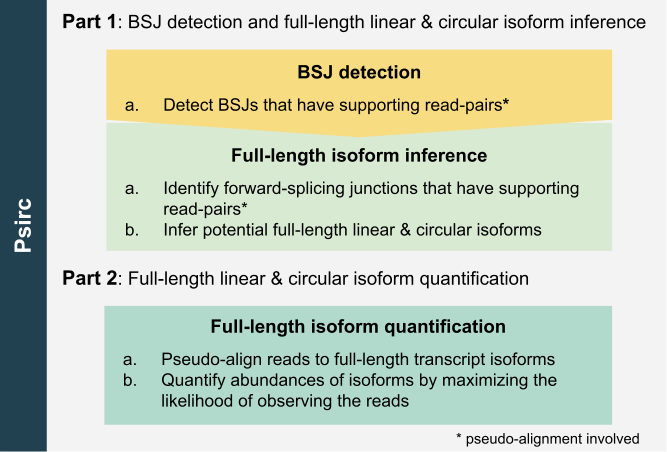
\includegraphics[width=0.5\textwidth]{chapters/3_materials_and_methods/figures/psirc_pipeline.png}
    \caption{psirc-workflow} \label{fig:psirc_workflow} \end{figure}

The initial phase of the workflow functions similarly to the implementation
described in \cref{sec:ciriquant}, with the added step of full-length isoform
inference.
However, this step requires paired-end sequencing data, which is not available
in this thesis.
While psirc's BSJ detection can be substituted with other tools, the FLI
inference step is more challenging to replace.
Previous studies have attempted to address this by using information from the
linear transcriptome to retain only exonic regions within the BSJ limits
\supercite{hoffmann_circrna-sponging_2023}.
If no exonic regions are present, the entire sequence is retained.
In contrast, the nf-core/circrna pipeline takes a different approach, retaining
the entire sequence within the BSJ boundaries, regardless of exonic region
presence.
This method avoids assumptions about the internal structure of the circRNA.

For the quantification phase, psirc requires a combined transcriptome FASTA
file containing both linear and circular transcripts.
Psirc constructs a Transcript de Bruijn Graph (T-DBG) from this combined
transcriptome and utilizes Kallisto to jointly quantify the expression levels
of both transcript types\supercite{yu_quantifying_2021}.
This approach enables a direct comparison between linear and circular isoforms,
potentially offering deeper insights into the regulatory roles of circRNAs in
gene expression.
Notably, psirc does not explicitly differentiate between reads spanning the BSJ
and those fully contained within it; instead, it relies on Kallisto's
likelihood maximization to distinguish between linear and circular
isoforms\supercite{yu_quantifying_2021}.